\documentclass[11pt]{article}
\usepackage{amsmath, amssymb, amscd, amsthm, amsfonts}
\usepackage{bm}
\usepackage{graphicx}
\usepackage{hyperref}

\usepackage{tikz}
\usepackage{pgfplots}
\usepackage{tabto}
\usepackage[siunitx]{circuitikz}
\usetikzlibrary{patterns, arrows, calc, decorations}
\usetikzlibrary{decorations.markings}
\usetikzlibrary{decorations.text}
\usepackage{hyperref}
\hypersetup{
  colorlinks=true,linkcolor=blue,urlcolor=cyan
}
\usepackage[portuguese]{babel} % Corrige linguaagem
\usepackage{svg}


\oddsidemargin 0pt
\evensidemargin 0pt
\marginparwidth 40pt
\marginparsep 10pt
\topmargin -20pt
\headsep 10pt
\textheight 8.7in
\textwidth 6.65in
\linespread{1.2}

\title{Eletro\'im\~as e suas aplicaç\~oes}
\author{Juan Vasconcelos, Matrícula: 201907140019 \and Jo\~ao Pedro Albuquerque, Matrícula: 201907140017 \and Jo\~ao Paulo de Andrade, Matrícula: 201907140009 \and Thiago Toni, Matrícula: 201907140061}
\date{}

\newtheorem{theorem}{Theorem}
\newtheorem{lemma}[theorem]{Lemma}
\newtheorem{conjecture}[theorem]{Conjecture}

\newcommand{\rr}{\mathbb{R}}

\newcommand{\al}{\alpha}
\DeclareMathOperator{\conv}{conv}
\DeclareMathOperator{\aff}{aff}

\begin{document}

\maketitle

\section{Introdução}\label{sec:introdução}
O estudo do eletromagnetismo gerou avanço em diversas áreas do conhecimento  como
medica, espacial e industrial e na vida cotidiana. Em aplicações cotidianas podemos
observar a presença do eletromagnéticos em aparelhos domésticos, sistemas de
comunicação e sistemas industriais, tais aplicações fazem uso de circuito magnético
para funcionamento que “consiste em uma estrutura que, em sua maior parte, é
composta por material magnético de permeabilidade elevada. A presença de um
material de alta permeabilidade tende a confinar o fluxo magnético aos caminhos
delimitados pela estrutura, do mesmo modo que, em um circuito elétrico, as correntes
são confinadas aos condutores”.

\section{Embasamento}\label{sec:embasamento}
O princípio de funcionamento de eletroímãs advem da Lei de Âmpère:
\begin{gather}
  \underbrace{ \oint_{\partial \Sigma} \bm{B} \cdot \: d{\bm{l}} }_\text{ campo magnético } = \mu_0 \left( \underbrace{ \iint_{\Sigma} \bm{J} \cdot \: d{\bm{S}} }_\text{corrente} + \underbrace{ \varepsilon \dfrac{d}{dt} \iint_{\Sigma} \bm{E} \: d{\bm{S}} }_\text{componente variante no tempo}  \right)
\end{gather}
ou igualmente em sua forma diferencial:
\begin{gather}
  \underbrace{\nabla \times \bm{B}}_\text{campo magnético} = \mu_0 \left( \underbrace{\bm{J}}_\text{corrente} + \underbrace{\varepsilon \dfrac{\partial \bm{E}}{\partial t}}_\text{componente variante no tempo} \right) 
\end{gather}

Ignorando por hora a componente variante no tempo, podemos nos focar no resultado
interessante para máquinas assíncronas: corrente elétrica em um condutor gera um
campo magnético, como ilustrado na figura~\ref{fig:sec:embasamento:1}. Enrolando
um condutor em forma helicoidal (um solenóide), que equivale a alinhar anéis em
sequência, teremos uma amplificação do campo, devido à contribuição de cada porção
de corrente no condutor, como ilustrado na figura~\ref{fig:sec:embasamento:2}

\begin{figure}
  \centering
\begin{tikzpicture}
  % anel com corrente
  \draw[
    decoration={markings, mark=at position 0 with {\arrow{<}}},
    decoration={markings, mark=at position 0.5 with {\arrow{<}}},
    postaction={decorate}
    ] (0,0,0) [y={(0,0,1)}] circle (1) node[above left] {};
  \node at (0,1.5,0) [y={(0,0,1)}] {$I$};
  
  % Campo magnético
  \draw[
    decoration={markings, mark=at position 0 with {\arrow{<}}},
    decoration={markings, mark=at position 0.5 with {\arrow{<}}},
    postaction={decorate}
    ] (1,0,0) [y={(0,1,0)}] circle (0.5);
  \node at (2,0,0) [y={(0,1,0)}] {$\bm{B}$};
  \draw[
    decoration={markings, mark=at position 0 with {\arrow{>}}},
    decoration={markings, mark=at position 0.5 with {\arrow{>}}},
    postaction={decorate}
    ] (-1,0,0) [y={(0,1,0)}] circle(0.5);
  \node at (-2,0,0) [y={(0,1,0)}] {$\bm{B}$};
  \draw[->] (0,-1,0) [y={(0,1,0)}] -- ++(0,2,0) node[left, near end]{$\bm{B}$};


  \draw[->] (-4,0,0) [y={(0,1,0)}] -- ++(0,1,0) node[left, near end]{$z$};
  \draw[->] (-4,0,0) [y={(0,0,1)}] -- ++(0,1,0) node[left, near end]{$x$};
  \draw[->] (-4,0,0) [y={(0,0,1)}] -- ++(1,0,0) node[above, near end]{$y$};
\end{tikzpicture}
\caption{Campo magnético atravessando um anel com corrente anti-horária}
\label{fig:sec:embasamento:1}
\end{figure}

\begin{figure}
  \centering
  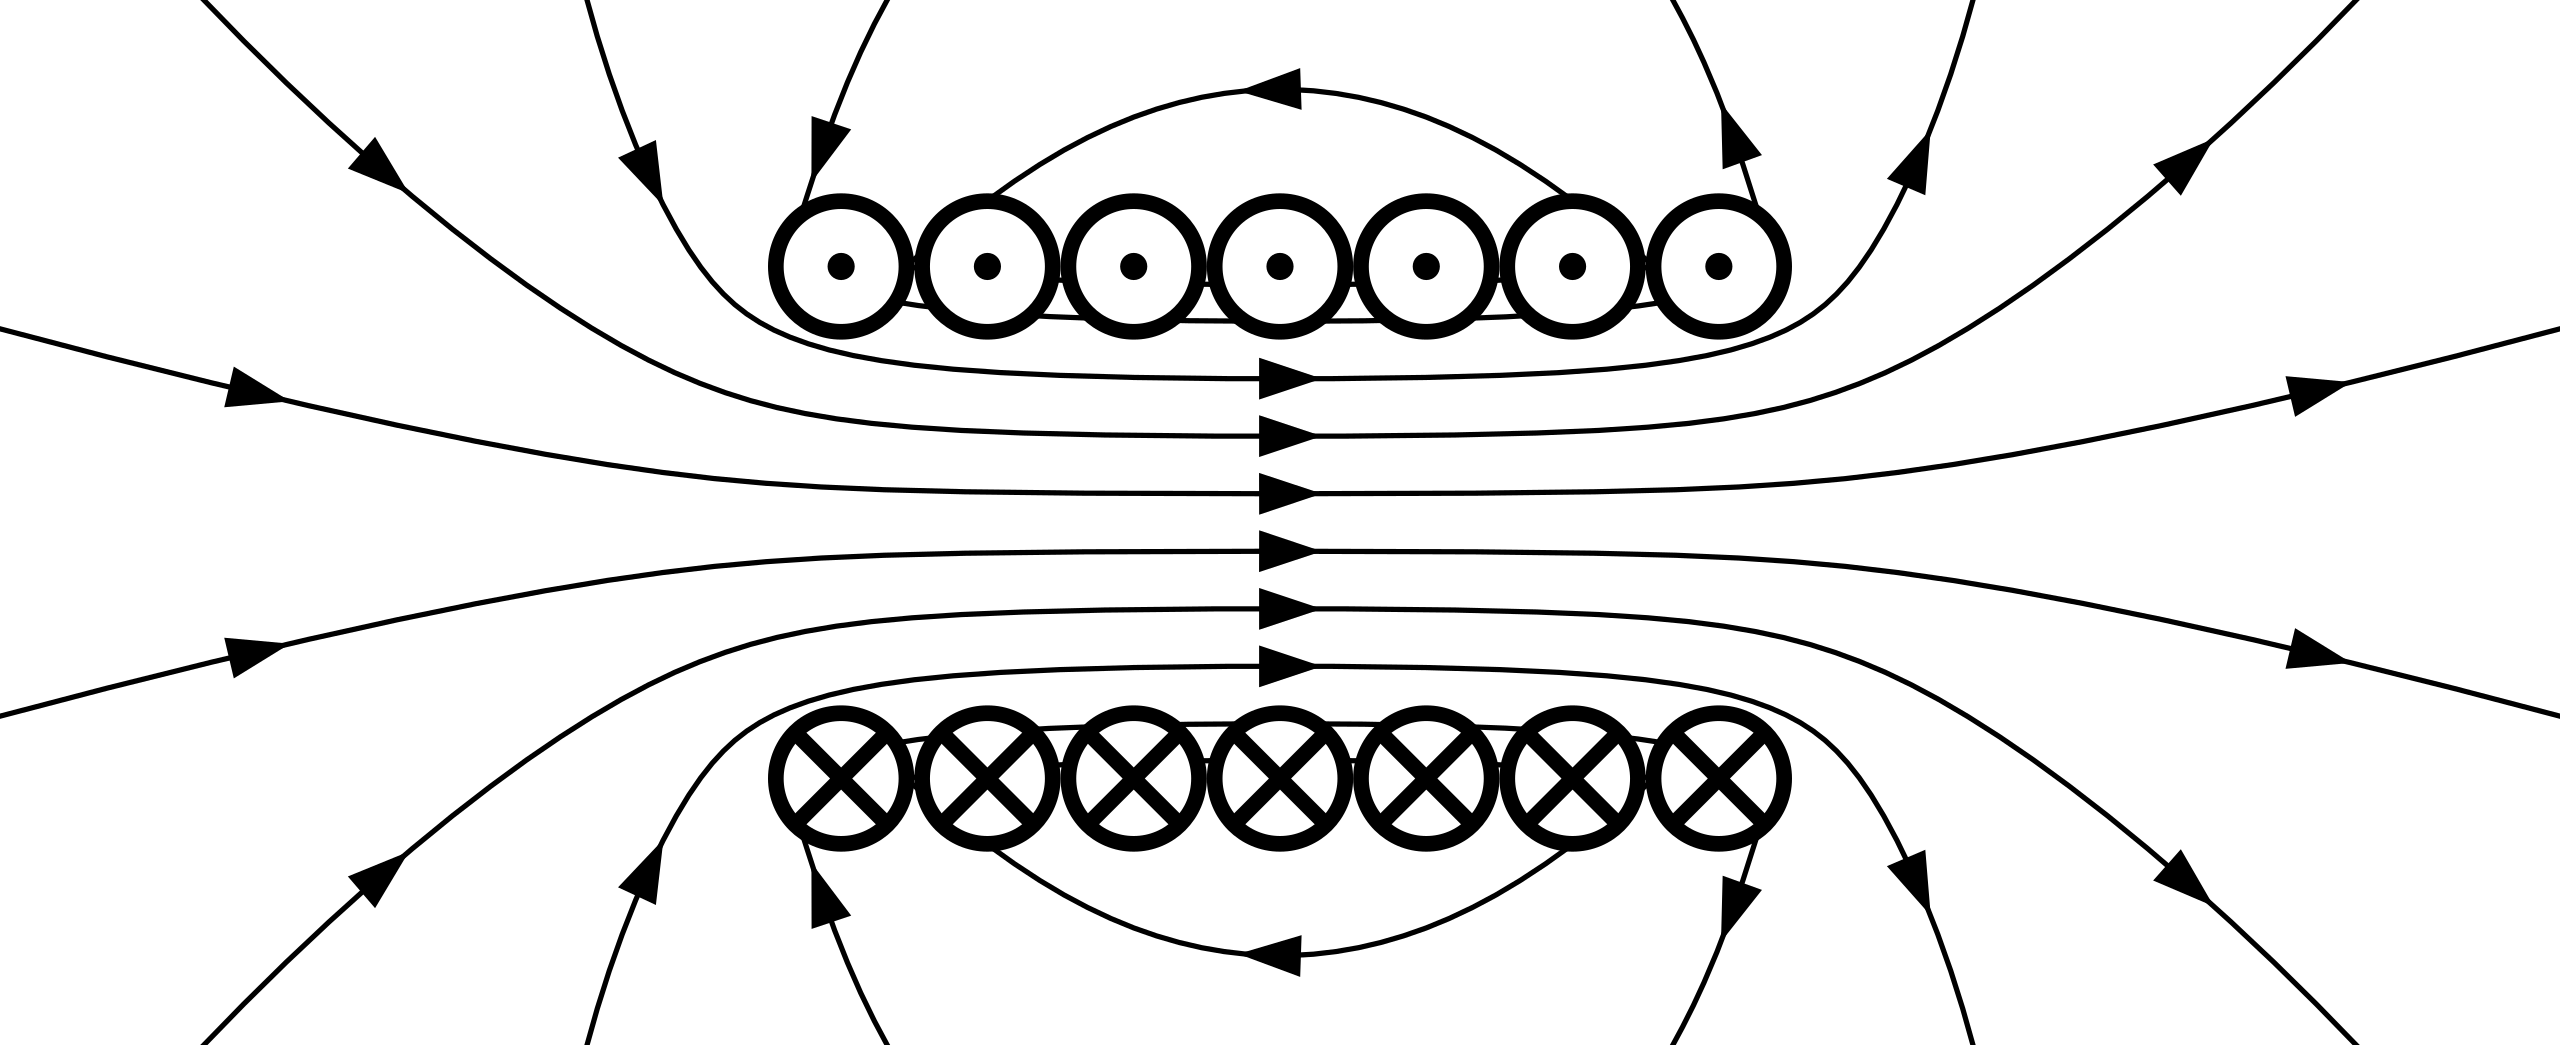
\includegraphics[width=0.5\columnwidth]{2560px-VFPt_Solenoid_correct2.svg.png}
  \caption{Campo magnético dentro de um solenóide}
  \label{fig:sec:embasamento:2}
\end{figure}

\begin{figure}
  \centering
  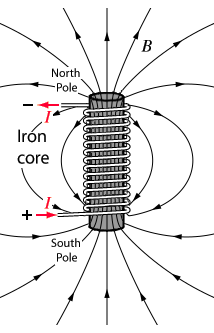
\includegraphics[width=0.2\columnwidth]{Elecmagnet.png}
  \caption{Solenoide amplificando o campo magnético no núcleo}
  \label{fig:sec:embasamento:3}
\end{figure}


\end{document}
